\section{Data}
To answer the challenge I need the following data points:
\medskip
\begin{enumerate}
  \item Number of inhabitants per province in the Netherlands
  \item Average house price per province in the Netherlands
  \item Number of restaurants per province in the Netherlands
\end{enumerate}
\medskip
Ad 1. The number of inhabitants per province in the Netherlands can be downloaded from the Centraal Bureau voor Statistiek \textbf{(CBS)}: a government owned, freely accessible web site with tons of statistical datasets (over 4K of them!) to use in all kind of analysis. I did some research on which table would best provide my need for the number of inhabitants per province and its title turns out to be \texttt{[Regionale kerncijfers Nederland]}. The resulting dataframe, including some data cleaning as removing substring \texttt{[(PV)]} from the province name.
\\\\
Ad 2. The average house price per province in the Netherlands in 2019 also can be downloaded from the CBS, this time based on the table with title \texttt{[Bestaande koopwoningen; gemiddelde verkoopprijzen, regio]}. After a bit of cleaning and tweaking (i.e. 'Friesland' ≠ 'Fryslân' and some column renaming had to be adjusted to make the dataset comprehensible for our international readers) the two dataframes could be joined.
\\\\
Ad 3. The third dataset, the number of restaurants, came from FourSquare. I needed to find all restaurants within each province of the Netherlands. The FourSquare API has the following two drawbacks that I needed to overcome: the non commercial API limits the returned venues per call to max 100 and although the results have a \texttt{[state]} field, the API doesn't allow searching per state. The limit of max 100 venues per call I overcame with the help of the material I found of a fellow course student Guillermo (G.) Bareirro \cite{STUDENT1}. FourSquare returns max 100 venues per call, but if you make the call specific enough, the total results will not grow above the limit. Using the categories listed bij G. Bareirro, I was able to split querying all restaurants into their separate categories and thereafter grouped and summed them with pandas standard dataframe functionality. 
\\\\
To overcome the second drawback of not being able to query FourSquare by state, I tried to find a geo boundaries source online of all the provinces in the Netherlands. Turned out there is no such source readably available in the public domain. Knowing that an estimate of the restaurants per province would be sufficient for my analyses, I queried the restaurants (via their respective subcategories) in the capital city of each province.
\\\\
The three data frames used in the analyses for this assignment are in the images below:
\medskip
\begin{figure}[h]
	\begin{subfigure}{0.33\textwidth}
		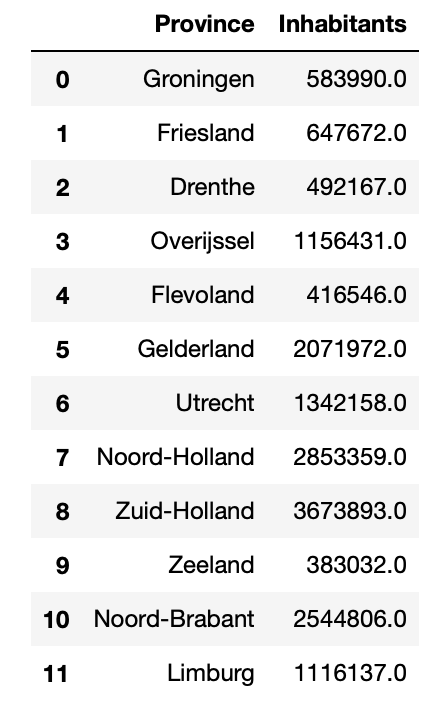
\includegraphics[scale=.4]{Inhabitants.png} 
		\caption{Inhabitants from StatLine \cite{CBS1}}
	\end{subfigure}
	\begin{subfigure}{0.33\textwidth}
		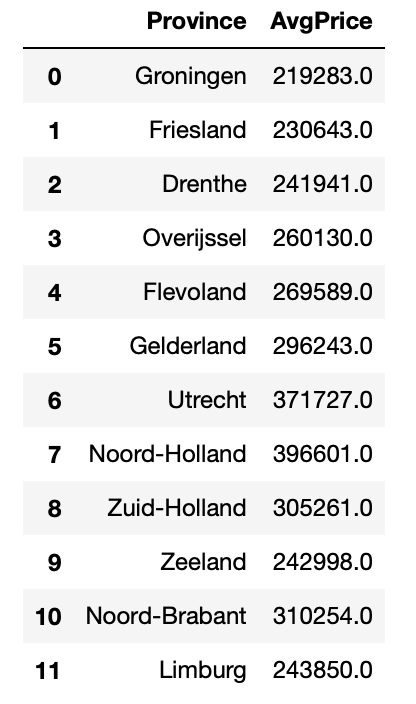
\includegraphics[scale=.4]{AvgPrice.png}
		\caption{Average Price from StatLine \cite{CBS2}}
	\end{subfigure}
	\begin{subfigure}{0.33\textwidth}
		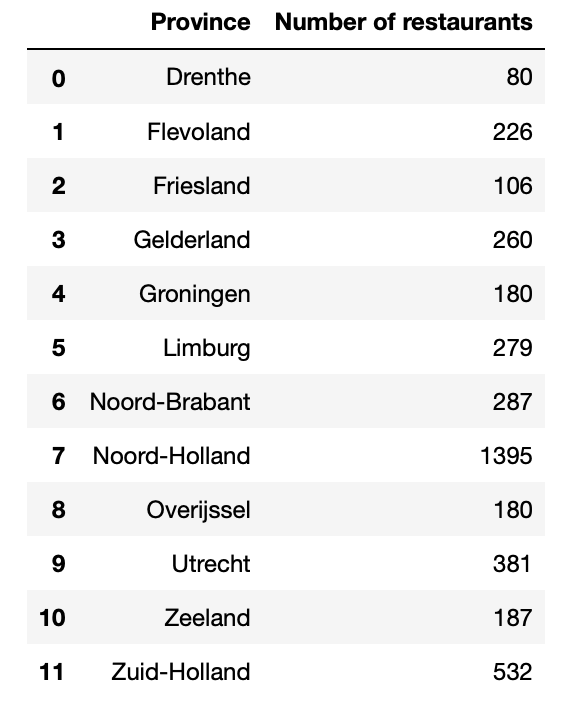
\includegraphics[scale=.4]{Restaurants.png}
		\caption{Restaurants from FourSquare \cite{FS2}}
	\end{subfigure}
\caption{Cleaned data frames as used in analysis}
\end{figure}